% ~~~~~~~~~~~~ %
% tab size = 4 %
% ~~~~~~~~~~~~ %

\documentclass[a4paper, 10pt, twocolumn, twoside]{article} % ~~~~~~ %
%																	%
% for IEEE articles ~ incompatibility with amsthm package			%
%\documentclass[letterpaper, 10 pt, conference]{ieeeconference} % ~ %
%\documentclass[letterpaper, 10 pt]{ieeetransactions} % ~~~~~~~~~~~ %
%\makeatletter														%
%\let\IEEEproof\proof												%
%\let\IEEEendproof\endproof											%
%\let\proof\@undefined												%
%\let\endproof\@undefined											%
%\makeatother														%
%																	%
\usepackage[latin1]{inputenc}										%
\usepackage[english]{babel}											%
\usepackage[T1]{fontenc}											%
\usepackage{dsfont}													%
\usepackage{booktabs}												%
\usepackage[table]{xcolor}											%
%\usepackage{makeidx}												%
\usepackage{fancyhdr}												%
\usepackage{lastpage}												%
\usepackage{amsmath, amssymb, amsfonts, amsthm}						% 
\usepackage[	left	= 2.5cm, right	= 2.5cm,					%
				bottom	= 2.5cm, top	= 2.5cm,					%
				bindingoffset	= 1cm]{geometry}					%
%																	%
\usepackage{ifpdf}													%
\ifpdf																%
	% ~~~~~~~~~~~~~~ if compiling with ``pdflatex'' ~~~~~~~~~~~~~~~ %
	%																%
	\usepackage[pdftex]{graphicx}									% 
	\DeclareGraphicsExtensions{.pdf,.png,.jpg,.mps}					%
	\usepackage[colorlinks,hyperindex,pagebackref=true]{hyperref}	%
	\pdfminorversion=6												%
\else																%
	% ~~~~~~~~~~~~~~~~ if compiling with ``latex'' ~~~~~~~~~~~~~~~~ %
	%																%
	\usepackage[dvips]{graphicx}									% 
	\usepackage[hyperindex]{hyperref}								%
\fi	% ~~~~~~~~~~~~~~~~~~~~~~~~~~~~~~~~~~~~~~~~~~~~~~~~~~~~~~~~~~~~~ %
%																	%
\usepackage{eso-pic}												%
\usepackage{tikz}				% (note: AFTER \pdfminorversion)	%
\usetikzlibrary{arrows,decorations.text,decorations.pathmorphing}	%
\usetikzlibrary{decorations.footprints,fadings,calc,trees,mindmap}	%
\usetikzlibrary{shadows,patterns,positioning,shapes,matrix,fit}		%
\usetikzlibrary{intersections}										%
\usepackage[switch, pagewise, mathlines]{lineno}					%
\usepackage[color=white!90!black, textwidth=3cm]{todonotes}			%
%																	%
\usepackage{algorithm}												%
\usepackage[noend]{algorithmic}										%
%																	%
% ~~~~~~~~~~~~~~~~~~~~~~~~~~~~~~~~~~~~~~~~~~~~~~~~~~~~~~~~~~~~~~~~~ %
%																	%
% in order to call \includegraphics{myImage}						%
% instead of \includegraphics{../images/myImage}					%
\graphicspath{{../Images/}}											%
%																	%
% ~~~~~~~~~~~~~~~~~~~~~~~~~~~~~~~~~~~~~~~~~~~~~~~~~~~~~~~~~~~~~~~~~ %


\newif\ifWorkingOnLinux
\newif\ifWorkingOnWindows
\newif\ifWorkingOnMac
%
\WorkingOnLinuxtrue
\WorkingOnWindowsfalse
\WorkingOnMacfalse


\pagestyle{fancy}
%
\fancyhead[LO]	{\slshape \leftmark}
\fancyhead[CO]	{}
\fancyhead[RO]	{\thepage \ on \pageref{LastPage}}
\fancyhead[LE]	{\thepage \ on \pageref{LastPage}}
\fancyhead[CE]	{}
\fancyhead[RE]	{\slshape \rightmark}
\fancyfoot[O]	{}
\fancyfoot[E]	{}

% --> numbered environments style ridefinition example:
%
%\newtheoremstyle{mystyle}	% name of the style
%{3pt}						% vertical space before the environment
%{8pt}						% vertical space after the environment
%{}							% body's font
%{}							% indentation (empty -> \parindent)
%{\bfseries}				% header's font
%{.}						% punctuation after the header
%{\newline}					% space after the header (empty -> \newline)
%{\thmname{#1}\thmnumber{ #2}\thmnote{ #3}}	% header formatting
%											% (cancel for the default)
%
%
% --> numbered environments ridefinition example
%
% \newtheorem	{unique_name}			% environment's ID
%										% (use \begin{unique_name})
%				[associated_counter]	% [optional] could be not
%										% unambiguous
%				{text}					% what will be printed
%				[sezione]				% [optional] to which kind of
%										% sectioning the enumeration
%										% will be tied
%
%
%
%
%
%
\newcounter{generalCounter}
\setcounter{generalCounter}{0}

\theoremstyle	{definition}
\newtheorem		{proposition}	[generalCounter]	{Proposition}
\newtheorem		{assumption}	[generalCounter]	{Assumption}
\newtheorem		{hypothesis}	[generalCounter]	{Hypothesis}
\newtheorem		{remark}		[generalCounter]	{Remark}
\newtheorem		{strategy}		[generalCounter]	{Strategy}
\newtheorem		{question}		[generalCounter]	{Question}
%
%
%
%
%
%
% usage example:
%
% \begin{theorem}[Pitagora]
% 	The square of...
% \end{theorem}



% ---------------------------------------------------------------------


% ----------------------------------------------------- % ------------------------------------------------------------
% \newcounter{nome_contatore}[contatore_gia_esistente]	% crea un contatore con il nome indicato,
% 														% il cui valore viene azzerato ogni volta che quello
% 														% opzionale (tra parentesi quadre) viene incrementato;
% ----------------------------------------------------- % ------------------------------------------------------------
% \setcounter{nome_contatore}{valore}					% assegna il valore indicato al contatore (deve
% 														% trattarsi di un valore intero, che eventualmente puo'
% 														% essere negativo);
% ----------------------------------------------------- % ------------------------------------------------------------
% \stepcounter{nome_contatore}							% incrementa il contatore di una singola unità e
% 														% azzera eventualmente i contatori che dipendono da questo;
% ----------------------------------------------------- % ------------------------------------------------------------
% \refstepcounter{nome_contatore}						% si comporta come \stepcounter, con la differenza che
% 														% coinvolge la creazione di un riferimento se seguito dal
% 														% comando \label;
% ----------------------------------------------------- % ------------------------------------------------------------
% \addtocounter{nome_contatore}{valore}					% aggiunge al contatore il valore indicato (deve
% 														% trattarsi di un valore intero, che eventualmente puo'
% 														% essere negativo);
% ----------------------------------------------------- % ------------------------------------------------------------
% \arabic{nome_contatore}								% traduce il valore del contatore in un numero arabo
% 														% nella composizione finale;
% ----------------------------------------------------- % ------------------------------------------------------------
% \thenome_contatore									% quando viene creato un contatore, si crea
% 														% implicitamente questo comando, con il quale si ottiene
% 														% il valore del contatore nella composizione finale,
% 														% espresso in modo predefinito (di solito si tratta di
% 														% un numero arabo);
% ----------------------------------------------------- % ------------------------------------------------------------
% \alph{nome_contatore}									% traduce il valore del contatore in una lettera
% 														% minuscola singola, pertanto si possono rappresentare
% 														% solo valori da 1 a 26;
% ----------------------------------------------------- % ------------------------------------------------------------
% \Alph{nome_contatore}									% traduce il valore del contatore in una lettera
% 														% maiuscola singola, pertanto si possono rappresentare
% 														% solo valori da 1 a 26;
% ----------------------------------------------------- % ------------------------------------------------------------
% \roman{nome_contatore}								% traduce il valore del contatore in un numero romano
% 														% con lettere minuscole, pertanto non si possono
% 														% rappresentare valori negativi;
% ----------------------------------------------------- % ------------------------------------------------------------
% \Roman{nome_contatore}								% traduce il valore del contatore in un numero romano
% 														% con lettere maiuscole, pertanto non si possono
% 														% rappresentare valori negativi;
% ----------------------------------------------------- % ------------------------------------------------------------
% \fnsymbol{nome_contatore}								% traduce il valore del contatore in un simbolo, ma
% 														% sono disponibili solo nove simboli, pertanto si
% 														% rappresentano valori da 1 a 9;
% ----------------------------------------------------- % ------------------------------------------------------------
% \value{nome_contatore}								% ottiene il valore del contatore, da usare all'interno
% 														% di un'espressione (non riguarda la composizione).
% ----------------------------------------------------- % ------------------------------------------------------------

\input{../Scripts/hyphenation}
\def\TITLE			{Presentation template}
\def\SHORTTITLE		{template}
\def\AUTHOR			{Author template}
\def\SHORTAUTHOR	{AT}
\def\INSTITUTE		{Institute template}
\def\SHORTINSTITUTE	{IT}
\def\SUBJECT		{Make a presentation template.}
\def\KEYWORDS		{Presentation, template}
\def\CREATOR		{University of template}
\def\DATE			{March 8 2010}
%
%
\def\THANKS
{
	\thanks
	{
		work supported by Uncle Duck
	}
}
%
\ifpdf \hypersetup
{
	pdftitle		= {\TITLE},
	pdfauthor		= {\AUTHOR},
	pdfsubject		= {\SUBJECT},
	pdfcreator		= {\CREATOR},
	pdfproducer		= {\INSTITUTE},
	pdfkeywords		= {\KEYWORDS},
	%
%	pdfpagemode		= FullScreen,		% se si vuole il full screen quando il documento viene aperto
	pdfstartview	= Fit,				% modalit� di visione del documento aperto (Fit FitH FitV FitR FitB)
	pdfstartpage	= 1,				% pagina su cui si vuole che venga aperto il file
	pdfnewwindow	= true,				% se si vuole che il pdf venga aperto su una finestra nuova
	pdfcenterwindow	= true,				% se si vuole che il pdf venga aperto al centro dello schermo
	pdftoolbar		= false,			% if you want to show Acrobat's toolbar
	pdfmenubar		= false,			% if you want to show Acrobat's menu
	%
	colorlinks		= false,			% false: boxed links    true: colored links
	linkbordercolor	= 0.8 0.8 0.8,		% (RGB) links normali
	citebordercolor	= 0.8 0.8 0.8,		% (RGB) links di citazione
	filebordercolor	= 0.8 0.8 0.8,		% (RGB) links ai files
	urlbordercolor	= 0.8 0.8 0.8,		% (RGB) links agli URL
}
%
\urlstyle{same}							% stile degli URL [same - commentato]
%
\fi
%
\title		[\SHORTTITLE]		{\TITLE}
\author		[\SHORTAUTHOR]		{\AUTHOR}
\date		{\DATE}
\institute	[\SHORTINSTITUTE]	{\INSTITUTE}
%
% if you want the current slide's index
%\author		[\SHORTAUTHOR \\ $\;$ \\ \insertframenumber $\;\!\!$ on \inserttotalframenumber]		{\AUTHOR}


% NOTE: hyperref could cause some warnings like:
%
%    ''Package hyperref Warning: Token not allowed in a PDFDocEncoded string:''
% 
% if you want to remove them you have to substitute the sentence using \texorpdfstring{}{} command like
% in the following example:
% \def\INSTITUTE
% {
%	\texorpdfstring
%	{Department of Information Engineering \\ University of Padova}		% actual TeX string
%	{Department of Information Engineering University of Padova}		% Bookmark used by hyperref
% }


\input{../Scripts/figuresgraphicalsettings}
\input{../Scripts/tablesgraphicalsettings}
% -------------------------------------------------------------------------
% theme settings
%\usetheme		[hideothersubsections,left,width=1.8cm]{Hannover}
\usetheme		[]{CambridgeUS}
\usefonttheme	[]{default}
\usecolortheme	[]{default}
\useinnertheme	[]{default}
\useoutertheme	[]{default}
%
% \setbeamercolor{structure}{fg = red}
% \setbeamercolor{structure}{bg = white}


% -------------------------------------------------------------------------
% Logo settings
\logo{\includegraphics[height = 1cm]{logo_dei__small}}


% -------------------------------------------------------------------------
% if you DO want the navigation symbols you have to comment the following line
\setbeamertemplate{navigation symbols}{}


% -------------------------------------------------------------------------
% set background as transparent
\setbeamercolor{background canvas}{bg = }


% -------------------------------------------------------------------------
% settings of the text to be unshown. Options:
% -> invisible	[text is invisible until it must appear]
% -> trasparent	[text is opaque (in %) until it must appear]
% -> dynamic	[text appears dynamically: initially invisible, then opaque and then appears fully]
\setbeamercovered{transparent=0}


% -------------------------------------------------------------------------
% if the frame is not fully occupied by text put the white space on the bottom
\raggedbottom


% -------------------------------------------------------------------------
% linespread definition
\linespread{1.1}


% -------------------------------------------------------------------------
% in order to remove some useless warnings
\let\Tiny=\tiny


% -------------------------------------------------------------------------
% measurement units:
%
% in - inches
% mm - millimeters
% cm - centimeters
% pt - points (about 1/72 inch)
% em - approximately the width of an "M" in the current font
% ex - approximately the height of an "x" in the current font 
%
% usage:
%\setlength{\thing_to_be_modified}{my_offset}
%
% modifiable things:
%
%--- Page Layout
%\columnsep:		gap between columns
%\topmargin:		gap above header
%\topskip:			between header and text
%\textheight:		height of main text
%\textwidth:		width of text
%\linewidth:		width of a line in the local environment
%\oddsidemargin:	odd page left margin
%\evensidemargin:	even page left margin
%\baselineskip:		normal vertical distance between lines in a paragraph
%\baselinestretch:	multiplies \baselineskip
%\voffset:
%
%--- Paragraphs
%\parindent:		indentation of paragraphs
%\parskip:			gap between paragraphs
%
%--- Floats (tables and figures)
%\floatsep:			space left between floats.
%\textfloatsep:		space between last top float or first bottom float and the text.
%\intextsep:		space left on top and bottom of an in-text float.
%\dbltextfloatsep:	is \textfloatsep for 2 column output.
%\dblfloatsep:		is \floatsep for 2 column output.
%\abovecaptionskip:	space above caption
%\belowcaptionskip:	space below caption
%\unitlength:		units of lenght in Picture Environment 
%
%--- Maths
%\abovedisplayskip:	space before maths
%\belowdisplayskip:	space after maths
%\arraycolsep:		gap between columns of an array
%
%--- Lists
%\topsep:			space between first item and preceding paragraph.
%\partopsep:		extra space added to \topsep when environment starts a new paragraph.
%\itemsep:			space between successive items.


% DECOMMENT THE PREFERRED OPTION



% -------------------------------------------------------------------
% image
%
% \setbeamertemplate{background}
% {
% 	\centering
% 	{
% 		\includegraphics[width=\paperwidth,height=\paperheight]{background_file.jpg}
% 	}
% }



% -------------------------------------------------------------------
% horizontal shading
%
% \pgfdeclarehorizontalshading
% {horizontal}					% name of the shading
% {2cm}							% shading height
% {	rgb(0cm)=(1.0, 1.0, 1.0);	% initial color
% 	rgb(1cm)=(1.0, 1.0, 0.8)}	% final color
%
% \AddToShipoutPicture
% {
% 	\begin{tikzpicture}[remember picture,overlay,shading=horizontal]
% 		\node (aa)	[xshift=-\textwidth,yshift=-\textheight]	at	(current page.south west)	{};
% 		\node (bb)	[xshift=+\textwidth,yshift=+\textheight]	at	(current page.north east)	{};
% 		\shade[shading angle=-90]	(aa)	rectangle	(bb);
% 	\end{tikzpicture}
% }



% -------------------------------------------------------------------
% radial shading
%
% \pgfdeclareradialshading
% {radial}						% nome
% {\pgfpoint{1.0cm}{0.7cm}}		% posizione del centro di illuminazione (0,0 � in mezzo alla sfera)
% {	rgb(0cm)=(0.9, 0.0, 0.0);	% colore iniziale
% 	rgb(2cm)=(0.5, 0.0, 0.0)}	% colore finale
%
% \AddToShipoutPicture
% {
% 	\begin{tikzpicture}[remember picture,overlay,shading=radial]
% 		\node (aa)	[xshift=-\textwidth,yshift=-\textheight]	at	(current page.south west)	{};
% 		\node (bb)	[xshift=+\textwidth,yshift=+\textheight]	at	(current page.north east)	{};
% 		\shade (aa)	rectangle	(bb);
% 	\end{tikzpicture}
% }



% -------------------------------------------------------------------
% text
%
% \AddToShipoutPicture
% {
% 	\begin{tikzpicture}[remember picture,overlay]
% 		\node [rotate=-60,scale=10,text opacity=0.1]
% 		at (current page.center)
% 		{For peer review only};
% 	\end{tikzpicture}
% }


\input{../Scripts/newcommands__estimations}

\newcommand{\DefinedAs}			[0]	{\mathrel{\mathop:}=}
\newcommand{\IDefinedAs}		[0]	{=\mathrel{\mathop:}}


\newcommand{\ExponentialOf}		[1]	{\mathrm{exp} \left( #1 \right)}
\newcommand{\LogarithmOf}		[1]	{\mathrm{log} \left( #1 \right)}
\newcommand{\ConvexHullOf}		[1]	{\mathrm{c.h.} \left( #1 \right)}


\newcommand{\MaximumOfOne}		[1]	{\mathrm{max} \left\lbrace #1 \right\rbrace}
\newcommand{\MaximumOfTwo}		[2]	{\mathrm{max} \left\lbrace #1, #2 \right\rbrace)}
\newcommand{\MaximumOfThree}	[3]	{\mathrm{max} \left\lbrace #1, #2, #3 \right\rbrace)}
\newcommand{\MinimumOfOne}		[1]	{\mathrm{min} \left\lbrace #1 \right\rbrace}
\newcommand{\MinimumOfTwo}		[2]	{\mathrm{min} \left\lbrace #1, #2 \right\rbrace)}
\newcommand{\MinimumOfThree}	[3]	{\mathrm{min} \left\lbrace #1, #2, #3 \right\rbrace)}


\newcommand{\CostFunction}				[0]	{Q}
\newcommand{\CostFunctionOf}			[1]	{\CostFunction \left( #1 \right)}
\newcommand{\CostFunctionOfSensor}		[1]	{\CostFunction_{#1}}
\newcommand{\CostFunctionOfSensorOf}	[2]	{\CostFunctionOfSensor{#1} \left( #2 \right)}


\newcommand{\KroneckerDeltaOf}			[2]	{\delta_{#1 #2}}


\newcommand{\FloorOf}			[1]	{\lfloor #1 \rfloor}
\newcommand{\CeilOf}			[1]	{\lceil #1 \rceil}
\newcommand{\SaturationOf}		[1]	{\mathrm{sat} \left( #1 \right)}
\newcommand{\PositivePartOf}	[1]	{\left[ #1 \right]_{+}}
\newcommand{\NegativePartOf}	[1]	{\left[ #1 \right]_{-}}


\newcommand{\GammaFunctionOf}	[1]	{\Gamma \left( #1 \right)}


\newcommand{\CholeskyFactorOf}	[1]	{\mathrm{chol} \left( #1 \right)}


\newcommand{\BigOOf}			[1]	{O \left( #1 \right)}

\input{../Scripts/newcommands__indices}
\newcommand{\IdentityMatrix}		[1]	{I_{#1}}
\newcommand{\OnesVector}			[1]	{\mathds{1}_{#1}}

\newcommand{\TraceOf}				[1]	{\mathrm{tr} \left( #1 \right)}
\newcommand{\DeterminantOf}			[1]	{\mathrm{det} \left( #1 \right)}

\newcommand{\Eigenvalue}			[0]	{\lambda}
\newcommand{\EigenvalueOfIndex}		[1]	{\Eigenvalue_{#1}}
\newcommand{\MaximalEigenvalue}		[0]	{\Eigenvalue_{\mathrm{max}}}
\newcommand{\MinimalEigenvalue}		[0]	{\Eigenvalue_{\mathrm{min}}}
\newcommand{\SetOfEigenvaluesOf}	[1]	{\mathrm{eig} \left( #1 \right)}

\newcommand{\Eigenvector}			[0]	{v}
\newcommand{\EigenvectorOfIndex}	[1]	{\Eigenvector_{#1}}

\newcommand{\SpectralRadius}		[0]	{\mu}
\newcommand{\SpectralRadiusOf}		[1]	{\SpectralRadius \left( #1 \right)}

\input{../Scripts/newcommands__probability_distributions}
\input{../Scripts/newcommands__set_theoretic_operators}
\input{../Scripts/newcommands__signals}
\input{../Scripts/newcommands__statistical_operators}
\input{../Scripts/newcommands__text}
\input{../Scripts/newcommands__networks}



% ~~~~~~~~~~~~~~~~~~~~~~~~~~~~~~~~~~~~~~~~~~~~~~~~~~~~~~~~~~~~~~~~~ %

%\makeindex

\begin{document}

%% for IEEE articles
%\IEEEoverridecommandlockouts    % for the \thanks
%\overrideIEEEmargins            % for the IEEE margins

%\setpagewiselinenumbers
%\modulolinenumbers[1]
%\linenumbers

%\maketitle						% print the standard LaTeX title
%% per non avere stili associati alla pagina corrente
\thispagestyle{empty}




% logo dell'universit�
\begin{center}
\includegraphics[width=2cm]{logo_unipd}
\label{fig:logo_unipd}
\end{center}




\vspace*{0.3cm}



\begin{center}
	UNIVERSIT\`A DEGLI STUDI DI $\ldots$\\
	DIPARTIMENTO DI INGEGNERIA DELL'INFORMAZIONE\\
\end{center}



\vspace*{1.2cm}


\begin{center}
{\color[rgb]{0.6,0.6,0.6} \rule[-1mm]{\textwidth}{0.2mm}}
\end{center}


\vspace*{0.6cm}


\begin{center}
\LARGE
{
	TITOLO \\
	DELL'OPERA
}
\end{center}


\vspace*{0.6cm}


\begin{center}
{\color[rgb]{0.6,0.6,0.6} \rule[-1mm]{\textwidth}{0.2mm}}
\end{center}


\vspace*{3cm}


\begin{center}

\includegraphics[height=2cm]{logo_dei_big}
\end{center}


\newpage
	% print the user defined title
%\tableofcontents				% print the table of contents
%\listoftables					% print the table of tables
%\listoffigures					% print the table of figures


%\begin{abstract}
Questo � un abstract.
\end{abstract}

%\section{Introduction}




\begin{frame}
	%
	\frametitle{Do you like$\ldots$ ?}
	%
	\begin{figure}[!htb]
\begin{center}
\begin{tikzpicture}
[
    xscale  = 1.0,
    yscale  = 1.0,
    transform canvas = {scale = 0.6},
    auto,
    %
    DecisionStyle/.style =
    {
        diamond,
        draw        = blue,
        thick,
        fill        = blue!20,
        text width  = 8em,
        align       = flush center,
        inner sep   = 1pt
    },
    %
    BlockStyle/.style =
    {
        rectangle,
        draw            = blue,
        thick,
        fill            = blue!20,
        text width      = 7.5em,
        align           = center,
        rounded corners,
        minimum height  = 2em
    },
    %
    CloudLineStyle/.style =
    {
        draw,
        ultra thick,
        color   = red,
        -latex,
        shorten >= 2pt,
        dotted
    },
    %
    BlockLineStyle/.style =
    {
        draw,
        ultra thick,
        color   = blue,
        -latex,
        shorten >= 2pt
    },
    %
    CloudStyle/.style =
    {
        draw            = red,
        thick,
        ellipse,
        fill            = red!20,
        minimum height  = 2em
    }
]



\matrix [column sep = 5mm, row sep = 7mm]
{
% row 1
\node [CloudStyle] (expert) {expert};           &
\node [BlockStyle] (init)   {initialize model}; &
\node [CloudStyle] (system) {system};           \\
%
% row 2
                                                            &
\node [BlockStyle] (identify)   {identify candidate model}; &
                                                            \\
%
% row 3
\node [BlockStyle] (update)     {update model};                 &
\node [BlockStyle] (evaluate)   {evaluate candidate models};    &
                                                                \\
%
% row 4
                                                                &
\node [DecisionStyle] (decide)  {is best candidate};            &
                                                                \\
% row 5
                                                                &
\node [BlockStyle] (stop)   {stop};                             &
                                                                \\
}; % end matrix



\draw   [BlockLineStyle]    (init)      -- (identify);
\draw   [BlockLineStyle]    (identify)  -- (evaluate);
\draw   [BlockLineStyle]    (evaluate)  -- (decide);
\draw   [BlockLineStyle]    (update)    |- (identify);
\draw   [BlockLineStyle]    (decide)    -| (update)     node [near start, color = black]    {yes} ;
\draw   [BlockLineStyle]    (decide)    -- (stop)       node [midway, color = black]        {no} ;
\draw   [CloudLineStyle]    (expert)    -- (init);
\draw   [CloudLineStyle]    (system)    -- (init);
\draw   [CloudLineStyle]    (system)    |- (evaluate);



\end{tikzpicture}
\end{center}
\end{figure}



	%
\end{frame}








\begin{frame}
	%
	\frametitle{\Tikz ist kein Zeichenprogramm}
	%
	\begin{center}
	\begin{tikzpicture}
		%
		\node [WarningTextStyle] {why should we use \Tikz for drawings?};
		%
	\end{tikzpicture}
	\end{center}
	%
	\uncover<1->
	{
		\alert{Advantages w.r.t.\ other drawing methods:}
		%
		\begin{itemize}
			\item extremely simple for logically simple drawings
			\item usage of \emph{native code} $\Rightarrow$ portable
			\item text and styles are the standard \LaTeX\ ones
			\item modification of existing drawings can be \alert{orders of magnitudo} more rapid (seconds vs.\ hours)
		\end{itemize}
	}
	%
\end{frame}





\begin{frame}
	%
	\frametitle{\Tikz ist kein Zeichenprogramm}
	%
	\begin{center}
	\begin{tikzpicture}
		%
		\node [WarningTextStyle] {why should we \textbf{\alert{do not}} use \Tikz for drawings?};
		%
	\end{tikzpicture}
	\end{center}
	%
	\uncover<1->
	{
		\alert{Disadvantages w.r.t.\ other drawing methods:}
		%
		\begin{itemize}
			\item quite slow when starting learning
			\item complicated for ``logically complicated'' pictures
			\item production of the first drafts can be \alert{orders of magnitudo} slower (hours vs.\ minutes)
		\end{itemize}
	}
	%
\end{frame}





\begin{frame}
	%
	\frametitle{General advice}
	%
	\uncover<1->
	{
		\begin{center}
		\begin{tikzpicture}
			%
			\node [WarningTextStyle]
			{read the chapter on ``Guidelines on Graphics'' on the \Tikz manual! (1.7)};
			%
		\end{tikzpicture}
		\end{center}
		%
		%
		general guidelines and principles concerning the \alert{creation of graphics for scientific presentations, papers, and books}
	}
	%
\end{frame}






\begin{frame}
	%
	\frametitle{Warning for the \LaTeX\ source code of this guide}
	%
	\begin{center}
	\begin{tikzpicture}
		%
		\node
		[WarningTextStyle]
		{In the \texttt{.tex} files of this presentation you may find someting like ``\texttt{uncover<1->}'': they are BEAMER commands, not \Tikz commands!!};
		%
	\end{tikzpicture}
	\end{center}
	%
	if you want to use this code you should cancel them
	%
\end{frame}





\begin{frame}
	%
	\frametitle{Where to obtain \Tikz}
	%
	\begin{description}
		%
		\item[stable version:]<1-> \texttt{pgf2.0} - official versions available in:
			%
			\vspace{0.3cm}
			%
			\begin{itemize}
				\item<1-> CTAN: \url{http://www.ctan.org/}
				\vspace{0.1cm}
				\item<1-> SourceForge: \url{http://sourceforge.net/projects/pgf/}
			\end{itemize}
		%
		\vspace{1.0cm}
		%
		\item[developement version:]<2-> \url{http://www.texample.net}
		%
	\end{description}
	%
\end{frame}





\begin{frame}
	%
	\frametitle{Where to obtain the developement version}
	%
	\begin{center}
	\begin{tikzpicture}
		%
		\uncover<1->
		{
			\node (nUrl) [sTextBlockStyle] {URL: \url{http://www.texample.net}};
		}
		%
		\uncover<2->
		{
			\node (nFirstSelect) [sTextBlockStyle, below = of nUrl] {select \Tikz};
			\draw [-open triangle 45, thick] (nUrl) to (nFirstSelect);
		}
		%
		\uncover<3->
		{
			\node (nSecondSelect) [sTextBlockStyle, below = of nFirstSelect] {download ``latest build''};
			\draw [-open triangle 45, thick] (nFirstSelect) to (nSecondSelect);
		}
		%
		\uncover<4->
		{
			\node (nInstallation) [sTextBlockStyle, below = of nSecondSelect]
				{install the (TDS-compliant) package};
			\draw [-open triangle 45, thick] (nSecondSelect) to (nInstallation);
		}
		%
		\uncover<5->
		{
			\node [sTextBlockStyle, below = of nSecondSelect, text = red, draw = red]
				{install the (TDS-compliant) package};
			\node (nQuestion) [below of = nInstallation] {don't know how? Google it!};
		}
		%
		%
	\end{tikzpicture}
	\end{center}
	%
\end{frame}




\begin{frame}
	%
	\frametitle{The most important advice:}
	%
	\uncover<2->
	{
		\begin{center}
		\begin{tikzpicture}
		[transform canvas = {scale = 1.5}]
				%
				\pattern
				[
					pattern color	= blue!25,
					pattern			= fivepointed stars,
					path fading	= middle,
				]
				(-5,-2) rectangle (5,2);
				%
				\node[color = red!90!black]
				{\Large{\textbf{\Tikz manual is your friend!}}};
				%
		\end{tikzpicture}
		\end{center}
	}
	%
\end{frame}




%\input{}
%\input{conclusions}


% ~~~~~~~~~~~~~~~~~~~~~~~~~~~~~~~~~~~~~~~~~~~~~~~~~~~~~~~~~~~~~~~~~ %
%																	%
\addcontentsline	{toc}{section}{References}						%
\bibliographystyle	{../Bibliography/ieeetransactions}				%
\bibliography		{../Bibliography/bibliography}					%
%\printindex														%
%\listoftodos														%
%																	%
% ~~~~~~~~~~~~~~~~~~~~~~~~~~~~~~~~~~~~~~~~~~~~~~~~~~~~~~~~~~~~~~~~~ %

\end{document}

% ~~~~~~~~~~~~~~~~~~~~~~~~~~~~~~~~~~~~~~~~~~~~~~~~~~~~~~~~~~~~~~~~~ %